\documentclass[11pt]{article}
\usepackage[latin2]{inputenc}
\usepackage{a4wide}
\usepackage{graphicx}
\usepackage{hyperref}
\hypersetup{colorlinks=true,linkcolor=blue}
\title{Assembly Documentation}
\author{ThingDoc}

\begin{document}

\maketitle
\begin{center}

\includegraphics[width=8cm]{logo.png}
\end{center}
Assembly of Low Profile Thumb Prosthesis

\newpage

\tableofcontents

\newpage

\section{Bill of Materials}
List of things you need to build the machine divided by categories.

\subsection{Prerequisites!}
\begin{itemize}
\item 4x 3D scan of patient's hand
\item 4x Configuration and Rendering of 3D models
\end{itemize}

\subsection{Materials}
\begin{itemize}
\item 100x \hyperlink{thing_g\_dragon\_skin\_30}{grams of Dragon Skin 30 liquid silicone}
\item 10x \hyperlink{thing_g\_dragon\_skin\_10}{grams of Dragon Skin 10 liquid silicone}
\end{itemize}

\subsection{Fasteners}
\begin{itemize}
\item 4x M4 Hex Nut
\item 1x \hyperlink{thing_velcro\_strap}{Velcro Strap}
\item 4x M4x15 Bolt
\end{itemize}

\subsection{Printed}
\begin{itemize}
\item 1x \hyperlink{thing_mold\_left\_half}{Mold - left half}
\item 1x \hyperlink{thing_truncated\_hand}{Truncated Print of Patient's Hand}
\item 1x \hyperlink{thing_rigid\_base}{Rigid base}
\item 1x \hyperlink{thing_mold\_right\_half}{Mold - right half}
\item 1x \hyperlink{thing_thumb\_with\_grip\_cutout}{Thumb with grip cutout}
\item 1x \hyperlink{thing_thumb\_mold}{Thumb Mold}
\end{itemize}

\newpage

\section{Things Overview}
List of things and their descriptions.

\hypertarget{thing_rigid\_base}{\subsection{Rigid base}}
3D printed rigid base for the static thumb post - rendered from src/scad/rigid_base.scad
\includegraphics[width=4cm]{images/rigid\_base.png}

\hypertarget{thing_silicone\_sleeve}{\subsection{Silicone sleeve}}
Silicone sleeve that goes over the patient's palm

\hypertarget{thing_molded\_thumb}{\subsection{Thumb with Molded Grip}}
Molded silicone thumb pad can improve grip and provide some tactile feedback to the wearer

\hypertarget{thing_truncated\_hand}{\subsection{Truncated Print of Patient's Hand}}
Shortened and resized portion of the patient's palm to be the center of the mold during silicone casting - rendered from src/scad/truncated_hand.scad (example shown)
\includegraphics[width=4cm]{images/truncated\_hand.png}

\hypertarget{thing_thumb\_mold}{\subsection{Thumb Mold}}
Mold for casting the silicone finger tip grip - rendered from src/inventor/thumb_mold.ipt
\includegraphics[width=4cm]{images/thumb\_mold.png}

\hypertarget{thing_g\_dragon\_skin\_10}{\subsection{grams of Dragon Skin 10 liquid silicone}}
Dragon Skin 10 silicone resin kit, available from Smooth-On. Shore A durometer (hardness) 10.
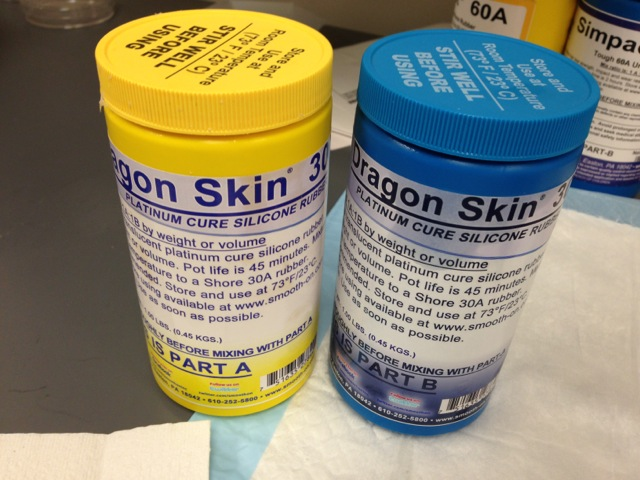
\includegraphics[width=4cm]{images/pad\_casting/DragonSkin.jpg}

\hypertarget{thing_thumb2}{\subsection{Thumb}}
Printed complete thumb without grip - rendered from src/inventor/thumb2.ipt

\hypertarget{thing_mold\_right\_half}{\subsection{Mold - right half}}
Right half of 3D printed mold for casting the silicone sleeve - rendered from src/scad/mold_right.scad
\includegraphics[width=4cm]{images/mold\_right\_half.png}

\hypertarget{thing_thumb\_with\_grip\_cutout}{\subsection{Thumb with grip cutout}}
Printed skeletal thumb tip - rendered from src/inventor/thumb_with_grip_cutout.ipt
\includegraphics[width=4cm]{images/thumb\_with\_grip\_cutout.png}

\hypertarget{thing_g\_dragon\_skin\_30}{\subsection{grams of Dragon Skin 30 liquid silicone}}
Dragon Skin 30 silicone resin kit, available from Smooth-On. Shore A durometer (hardness) 30.
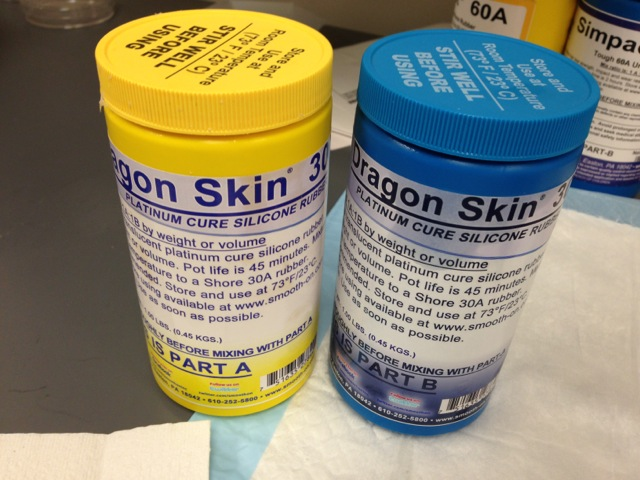
\includegraphics[width=4cm]{images/pad\_casting/DragonSkin.jpg}

\hypertarget{thing_velcro\_strap}{\subsection{Velcro Strap}}
9mm wide velcro strap of adequate length to wrap around the patient's palm with at least 30% extra.

\hypertarget{thing_mold\_left\_half}{\subsection{Mold - left half}}
Left half of 3D printed mold for casting the silicone sleeve - rendered from src/scad/mold_left_half.scad
\includegraphics[width=4cm]{images/mold\_left\_half.png}

\hypertarget{thing_mold\_assembly}{\subsection{Palm Sleeve Mold Assembly}}
Assembled mold for casting the silicone sleeve

\newpage

\section{Assembly Instructions}

\subsection{Assemble Configuration and Rendering of 3D models}
Things needed:
\begin{itemize}
\item 1x 3D scan of patient's hand
\end{itemize}
Steps:
\begin{enumerate}
\item Open configuration.scad in your favorite text editor.
\item Set the variables (more documentation coming soon!)
\item Render each part (F6) and export as STL, then print.
\end{enumerate}

\subsection{Assemble Configuration and Rendering of 3D models}
Things needed:
\begin{itemize}
\item 1x 3D scan of patient's hand
\end{itemize}
Steps:
\begin{enumerate}
\item Open configuration.scad in your favorite text editor.
\item Set the variables (more documentation coming soon!)
\item Render each part (F6) and export as STL, then print.
\end{enumerate}

\subsection{Assemble Configuration and Rendering of 3D models}
Things needed:
\begin{itemize}
\item 1x 3D scan of patient's hand
\end{itemize}
Steps:
\begin{enumerate}
\item Open configuration.scad in your favorite text editor.
\item Set the variables (more documentation coming soon!)
\item Render each part (F6) and export as STL, then print.
\end{enumerate}

\subsection{Assemble Palm Sleeve Mold Assembly}
Things needed:
\begin{itemize}
\item 1x \hyperlink{thing_rigid\_base}{Rigid base}
\item 1x \hyperlink{thing_mold\_left\_half}{Mold - left half}
\item 4x M4x15 Bolt
\item 1x \hyperlink{thing_mold\_right\_half}{Mold - right half}
\item 4x M4 Hex Nut
\end{itemize}
Steps:
\begin{enumerate}
\item Set one half of the mold on a flat surface with the flat side down.
\item Insert the rigid thumb base into the slot in the side of the mold, with the round part towrd the inside and the shorter prong toward the closed end of the mold.
\item Set the other half of the mold with the flat side up so the two halves align.
\item Fasten the two halves together using the nuts and bolts in the holes at each corner.
\end{enumerate}

\subsection{Assemble Configuration and Rendering of 3D models}
Things needed:
\begin{itemize}
\item 1x 3D scan of patient's hand
\end{itemize}
Steps:
\begin{enumerate}
\item Open configuration.scad in your favorite text editor.
\item Set the variables (more documentation coming soon!)
\item Render each part (F6) and export as STL, then print.
\end{enumerate}

\subsection{Assemble Silicone sleeve}
Things needed:
\begin{itemize}
\item 100x \hyperlink{thing_g\_dragon\_skin\_30}{grams of Dragon Skin 30 liquid silicone}
\item 1x \hyperlink{thing_mold\_assembly}{Palm Sleeve Mold Assembly}
\item 1x \hyperlink{thing_truncated\_hand}{Truncated Print of Patient's Hand}
\end{itemize}
Steps:
\begin{enumerate}
\item Mix silicone according to the instructions from the supplier. Wear gloves and follow the supplier's safety guidelines while working with liquid silicone.\\ 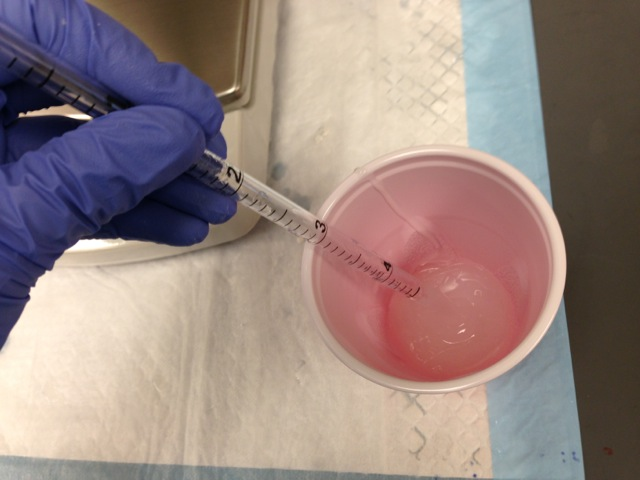
\includegraphics[width=4cm]{images/pad\_casting/Mixing.jpg}
\item Pour the liquid silicone to about halfway fill the mold.
\item Insert the truncated hand in the opening of the mold, narrow side down, so that it sits in the center of the mold and lines up with the overall shape of the mold. Make sure there is a small gap between the truncated hand and the thumb base piece.
\item Make sure the silicone settles to the bottom and that there is enough to fill the mold completely.
\item After the silicone cures, unscrew and separate the two halves of the mold, and pull out the truncated hand.
\item If necessary, use a knife to cut off any excess silicone and/or cut to better fit the patient's hand.
\end{enumerate}

\subsection{Assemble Thumb with Molded Grip}
Things needed:
\begin{itemize}
\item 10x \hyperlink{thing_g\_dragon\_skin\_10}{grams of Dragon Skin 10 liquid silicone}
\item 1x \hyperlink{thing_thumb\_mold}{Thumb Mold}
\item 1x \hyperlink{thing_thumb\_with\_grip\_cutout}{Thumb with grip cutout}
\end{itemize}
Steps:
\begin{enumerate}
\item Print the skeletal thumb tip and mold.
\item Mix silicone according to the instructions from the supplier. Wear gloves and follow the supplier's safety guidelines while working with liquid silicone.\\ 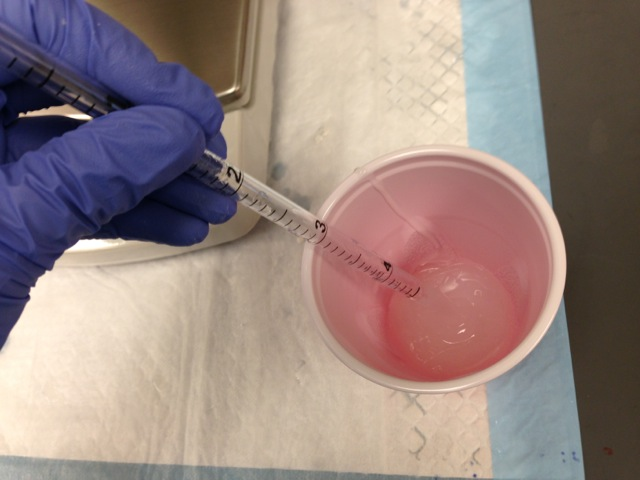
\includegraphics[width=4cm]{images/pad\_casting/Mixing.jpg}
\item Pour the liquid silicone to mostly fill the thumb mold.
\item Insert the printed skeletal thumb into the filled mold as far as it will go.
\item Remove most of the excess silicone. Small amounts of excess can be removed afer molding.
\item After the silicone has cured, carefully pull the thumb to remove it from the mold.
\item If necessary, use a knife to trim off excess silicone so that the edges of the silicone part are flush with those of the hard printed part.
\end{enumerate}

\subsection{Assemble Assembly}
Things needed:
\begin{itemize}
\item 1x \hyperlink{thing_silicone\_sleeve}{Silicone sleeve}
\item 1x \hyperlink{thing_molded\_thumb}{Thumb with Molded Grip}
\item 1x \hyperlink{thing_velcro\_strap}{Velcro Strap}
\end{itemize}
Steps:
\begin{enumerate}
\item Insert the thumb into the slot on the base.
\item Insert the velcro strap through the slot on the base.
\item Insert patient's hand into the sleeve.
\item Fasten the velcro strap and tighten as needed to hold the prosthesis in place during use.
\end{enumerate}

\newpage

\end{document}